% Technical report (English). Build: bash docs/report/build.sh
\documentclass[10pt,a4paper,twocolumn]{article}
\usepackage[margin=17mm,columnsep=6mm]{geometry}
\usepackage{amsmath,amssymb}
\usepackage{booktabs}
\usepackage{graphicx}
\usepackage{xcolor}
\usepackage{tikz}
\usetikzlibrary{positioning,arrows.meta,fit,calc}
\usepackage[font=small,labelfont=bf]{caption}
\usepackage{enumitem}
\setlist{nosep,leftmargin=*}
\usepackage{xeCJK}
\setCJKmainfont[Path=fonts/,BoldFont=NotoSerifJP-Bold.otf]{NotoSerifJP-Regular.otf}
\usepackage[colorlinks=true,linkcolor=blue!50!black,citecolor=blue!50!black,urlcolor=blue!50!black]{hyperref}
\newcommand{\pt}{\,pt}
\setlength{\emergencystretch}{1.5em}

\title{\bfseries Pocket TTS Learns Japanese:\\
Training Data and Distillation for a Drop-in 100M-Parameter Model}
\author{Claude (Anthropic)\thanks{Claude (Opus 5.5), working in Claude Code, planned and implemented
the data pipeline and the experiments, ran them, analyzed the results and wrote this report; a second
Claude Code session did the decoder fine-tuning of \S\ref{sec:decoder}. Takuma Mori set the goals (a
Japanese model that the stock \texttt{pocket-tts} package loads unchanged, and a second line trained on
CC BY data only), chose the data sources and their licenses, provided the machines, did the listening
tests (which found the extra speech after short sentences and chose the decoders) and decided the
releases.}\qquad Takuma Mori}
\date{{\small Technical report, October 2026}\\
{\small\url{https://github.com/takuma104/pocket-tts-ja}}}

\begin{document}
\maketitle

\begin{abstract}
Pocket TTS is a 100M-parameter text-to-speech (TTS) model from Kyutai that runs faster than real
time on a laptop CPU: a causal transformer predicts the continuous latents of the Mimi codec, and a
small flow head samples each 80\,ms frame in one step. We adapt it to Japanese under a strict
constraint: the result must load in the stock \texttt{pocket-tts} package through a config file,
read plain kanji--kana text without a pronunciation front end, and keep zero-shot voice cloning.
Most of the work went into the training data. We filter web speech (Emilia, YODAS3) with ASR
re-checks, restore punctuation, match loudness with per-speaker gain copies, and cover rare kanji
readings with 0.4--0.8\,kh of synthetic speech whose readings an ASR model confirmed. Accuracy
follows how often a reading occurs in training, and new synthetic data, not more steps, broke every
plateau. The stock runtime generates a few frames after the end-of-speech decision that upstream
training never supervises; supervising them with digital silence removed fillers that followed
about 10\% of the sentences. Guidance is distilled into the weights, and a 6-layer student reads
better than its 24-layer teacher. Finally, only the codec's decoder is fine-tuned, so latents and
voice prompts stay compatible. On the 13,536 sentences of JKYB-Parakeet, the released 6-layer models
read 94.75\% (trained with Emilia, CC BY-NC) and 94.77\% (CC BY data only) of the target words
correctly.
\end{abstract}

\section{Introduction}
Pocket TTS~\cite{pocket} is a small TTS model released by Kyutai in 2026 and built on continuous
audio language models (CALM)~\cite{calm}. It has about 100M parameters, streams with about 200\,ms of
latency, runs about 6$\times$ faster than real time on two laptop CPU cores, and clones a voice from
a few seconds of audio. Kyutai publishes its training code, including a recipe for new languages. The
official models cover English and six European languages; none covers Japanese.

Japanese is hard for such a model. Text has no spaces, and most kanji have several readings that
depend on the word and the context: 生 is \emph{sei} in 生活, \emph{nama} in 生ビール and \emph{i}
in 生きる. Pocket TTS has no text encoder and no dictionary: a lookup table embeds the tokenizer's
pieces, and the transformer must learn every reading from paired speech, in which rare readings
occur only a few times.

Our goals were: (i)~the model loads in the stock package (3.3.0) with \texttt{--config} and no code
changes; (ii)~it reads plain Japanese text; (iii)~a 6-layer model runs on CPU; (iv)~besides a line
trained with the non-commercial Emilia corpus (the \emph{main line} below), a second line, the
\emph{CC BY line}, uses CC BY data only, so that its weights can be used commercially. We describe the training data (\S\ref{sec:data}), the training
recipe and the supervision of the utterance end (\S\ref{sec:train}), distillation (\S\ref{sec:distill}),
the decoder (\S\ref{sec:decoder}) and the released models (\S\ref{sec:results}), which are on Hugging
Face\footnote{\url{https://huggingface.co/takuma104/pocket-tts-ja} (CC BY-NC 4.0) and
\url{https://huggingface.co/takuma104/pocket-tts-ja-cc} (CC BY 4.0).}.

\section{Pocket TTS}\label{sec:arch}
\textbf{FlowLM.} A causal transformer (6 or 24 layers, width 1024, 16 heads) reads the conditioning
and then the target latents frame by frame. Its output conditions a flow head, an MLP with adaptive
layer norm (6 blocks, width 512)~\cite{mar} trained with Lagrangian self-distillation
(LSD)~\cite{lsd}, a consistency-style objective. Inference takes one step,
$x_1=x_0+v(0,1,x_0)$ with $x_0\sim\mathcal{N}(0,\tau)$ and temperature $\tau=0.3$. A linear head on
the transformer output predicts the end of speech (EOS). The sequence is a learned token, the voice
prompt (projected Mimi latents of the reference audio), the text (one embedding per piece), a BOS
latent and the target. Training drops the text and the voice 20\% of the time each, for
classifier-free guidance (CFG)~\cite{cfg} on the transformer output.

\textbf{Mimi}, the codec of Moshi~\cite{moshi}, encodes 24\,kHz audio into 32-dimensional continuous
latents at 12.5\,Hz with a convolutional SEANet encoder and decoder (strides 6, 5, 4) and small
transformers. It is frozen and the same in every language release (Table~\ref{tab:arch}).

\begin{table}[t]
\centering\footnotesize\setlength{\tabcolsep}{3pt}
\caption{Parts of Pocket TTS (6- / 24-layer models) and what this work trains ($^\ast$frozen during
distillation).}
\label{tab:arch}
\begin{tabular}{@{}lrl@{}}
\toprule
Part & Params & This work\\
\midrule
Transformer (width 1024) & 75.5M / 302.1M & trained\\
Text table (4,000 pieces) & 4.1M & new\\
Flow head, EOS head & 9.8M & trained$^\ast$\\
Mimi encoder side & 9.8M & frozen\\
Mimi decoder side & 10.3M & fine-tuned (\S\ref{sec:decoder})\\
\midrule
Total & 109.5M / 336.1M &\\
\bottomrule
\end{tabular}
\end{table}

\textbf{What the stock runtime fixes.} The config sets the weights, the sizes, the SentencePiece
tokenizer, the temperature, text replacements and the number of frames after EOS. The rest is
fixed: there is no CFG; text is cut into chunks of at most 50 tokens at sentence, then clause
punctuation; generation stops at $\text{tokens}/3+2$\,s; the tokenizer does no normalization. After
EOS the runtime generates 3 more frames for inputs of up to four space-separated words (else 1),
plus 2, so a Japanese sentence, one ``word'', gets 5 frames (400\,ms). These rules explain a small
vocabulary, ASCII punctuation in training, distilled CFG, and our care for short chunks and the
frames after EOS.

\section{Training data}\label{sec:data}
\subsection{Natural speech}
\textbf{Emilia}~\cite{emilia,emilialarge} has 1,716\,h (Emilia, CC BY-NC) and 1,120\,h (Emilia-YODAS,
CC BY) of Japanese 3--30\,s clips. Three Emilia shards are 95\% byte-identical to Emilia-YODAS, and
21\% of the rest are duplicates (re-uploaded listening drills, channel outros). A speaker label is one
diarized speaker in one video (ECAPA~\cite{ecapa} similarity 0.69--0.73 within a label, 0.15 across),
so the voice prompt, which must be another utterance of the target speaker, is taken from the same
label. After de-duplication and filters (1.5--15 characters/s, DNSMOS~\cite{dnsmos} $\ge$3.0, no
benchmark sentences, $\ge$2 utterances per speaker, speaker consistency), 1,709\,h remain.

\textbf{YODAS3}~\cite{yodas,yodas3} (CC BY 3.0) has 17,404\,h of full-band Japanese YouTube audio with
no segments, speakers or quality scores and mostly automatic captions without punctuation. We cut
3--20\,s utterances at pauses (Silero VAD~\cite{silero}), transcribe them with Whisper~\cite{whisper}
and keep an utterance when the readings of caption and transcript agree (kana CER $\le$0.10 without
fillers); the transcript is the label. Speakers are per-video ECAPA clusters; a cluster that matches
clusters in $\ge$20 other videos is a mass-produced TTS voice (in a pilot, all were Wikipedia read by
TTS) and is dropped. Of 8,311\,h of segments, 601\,h remain. 72\% of the labels had no punctuation
(Emilia 2--7\%), which teaches pauses without commas; transcribing each clip again with a punctuated
prompt and copying only the punctuation leaves 1.3\% without.

\subsection{What listening and ASR found}\label{sec:found}
\textbf{Speech after short sentences.} Listening found junk after short sentences
(…ハチガツデス、ゲツ): 26--44\% of the JKYB sentences under 15 kana ended with two or more extra kana,
none above 30. The shortest Emilia clip is 3.04\,s, so short transcripts sit in long clips (2.2
against 5.6 characters/s), and in 40\% of those we heard, the speaker repeated the sentence or kept
talking. We decode the exact training latents, transcribe them with kana-whisper~\cite{kanawhisper}
and drop a clip if the ASR inserts $\ge\max(3,0.2n)$ kana after removing fillers ($n$: reference
kana), the CER exceeds 0.3 or the ASR loops. Emilia keeps 1,531\,h, and with short Tatoeba sentences
(S4 below), extra speech after sentences under 15 kana fell from 25.8\% to 3.0\%. On YODAS3 the
check dropped half of the clips under 15 kana (559\,h remain).

\textbf{Loudness.} Quiet prompts gave quiet outputs: training audio sits at $-24$ to $-14$\,LUFS,
JVS prompts at $-24$ to $-31$, and the runtime does not normalize prompts. We re-encode 20\% of the
Emilia clips with a per-speaker gain from $[-15,+3]$\,dB, as separate speakers so that prompt and
target share it (227\,h); the loudness gap to the prompt went from $-2.2$ to $-0.9$\,LU.

\subsection{Reading-rich synthetic speech}
\textbf{Why.} With Emilia only, the teacher stalled at 70--72\% on JKYB-mini. Accuracy follows the
exposure of a kanji--reading pair, the number of training sentences that contain it: 32\% for 1--9,
54\% for 10--29, 83\% for 30--99, 89\% for 100--299 and 95--96\% above. Writing the target in
katakana raised accuracy from 88.1\% to 96.2\%: the model can say the readings but lacks the mapping
from kanji.

\textbf{Teacher and texts.} We synthesize with Irodori-TTS-v4.1-Small-Yomi~\cite{yomi}, whose kanji
readings we had improved by text-only self-distillation (JKYB 95.7\%, MIT license), in 3,000 voices
from Emilia. The first 300k sentences (S1) are the reading-targeted sentences of that work
(KANJIDIC2~\cite{jmdict}, Aozora Bunko ruby, LLM sentences), Wikipedia sentences with words rare in
Emilia, and general sentences. No word was chosen with the benchmark's keys, and sentences that
overlap JKYB, JVS, JSUT or the Aozora evaluation works were removed.

\textbf{Quality control and its bias.} A clip is kept only if kana-whisper reads every target exactly
and the sentence CER is $\le$0.08. This removes exactly the hard cases: of 120k rejected S3
sentences, 84k failed because Irodori itself misread the target. Set S5 re-synthesizes them with the
target written in katakana, keeping the kanji transcript. Later sets top up readings that stayed rare
(Table~\ref{tab:synth}).

\begin{table}[t]
\centering\footnotesize\setlength{\tabcolsep}{3pt}
\caption{Synthetic sets of the main line. Kept: passed the ASR check of every target and of the
sentence.}
\label{tab:synth}
\begin{tabular}{@{}llrr@{}}
\toprule
Set & Texts & Kept & Hours\\
\midrule
S3 & S1 (targeted, Wikipedia, general) & 179k (60\%) & 341\\
S4 & Tatoeba, 2--20 characters & 21k (54\%) & 19\\
S5 & S3 rejects, target in katakana & 43k (55\%) & 84\\
S6a/b & Wikipedia, readings to 300 sentences & 108k (72\%) & 215\\
S7 & LLM sentences, rare readings$^\ast$ & 13k (82\%) & 15\\
S9 & 2--8 tokens, explicit duration & 31k (69\%) & 11\\
\bottomrule
\end{tabular}\\[2pt]
{\footnotesize $^\ast$Written by Claude Haiku; homographs checked by Claude Sonnet.}
\end{table}

\textbf{Effect.} Each set moved the plateau (Fig.~\ref{fig:training}). 10\% of S3 took JKYB-mini
from 72.3\% to 77.2\% within 7k steps (JSUT CER 6.95$\to$5.36\%). S7 raised the readings it topped up
with $\ge$10 sentences from 53\% to 80\%; readings it did not touch stayed at 50\%. S6a and S5
followed (91.0\%, 91.8\%). Speaker similarity did not change with 22--31\% synthetic data. The CC
BY line used the synthetic sets from early in training: the 309k sentences that had passed in Emilia
(NC) voices were synthesized again with the same text and seed in Emilia-YODAS voices (2,998 voices,
553\,h).

\subsection{Text, tokenizer and mixes}
Text is normalized (NFKC, 。$\to$\texttt{.}, 、$\to$\texttt{,}, no brackets, a space after each
sentence end, as the runtime joins chunks with spaces), and 124 replacement rules in the config do the
same at inference. The tokenizer is a 4,000-piece SentencePiece unigram model~\cite{sentencepiece}
trained on the transcripts. Against 8,000 pieces it read better after 15k steps (65.3 vs 63.4\%,
McNemar $p=0.031$), and its 50-token chunks fit the length limit more often. The runtime may generate
a sentence's last clause alone, but only 0.04\% of the training utterances have five tokens or
fewer, and Irodori stretches very short texts to 2--3\,s; S9 synthesizes 2--8-token texts with an
explicit duration (0.13\,s per mora). Table~\ref{tab:mix} gives the final mixes. A script checks every
row of the CC BY mixes against the source manifests: none comes from the NC part of Emilia, directly
or as a synthetic voice.

\begin{table}[t]
\centering\footnotesize\setlength{\tabcolsep}{3pt}
\caption{Training mixes of the released teachers (hours). NC: CC BY-NC 4.0; BY: CC BY ($^\ast$by the
reference voices).}
\label{tab:mix}\setlength{\tabcolsep}{2.3pt}
\begin{tabular}{@{}lrrl@{}}
\toprule
Source & Main & CC BY & License\\
\midrule
Emilia (CC BY: Emilia-YODAS only) & 1,531 & 305 & NC / BY\\
\quad gain copies & 227 & 48 &\\
YODAS3 & -- & 556 & BY 3.0\\
Synthetic (Irodori-TTS) & 828 & 425 & NC / BY$^\ast$\\
\midrule
Total & 2,592 & 1,334 &\\
\bottomrule
\end{tabular}
\end{table}

\section{Training the teacher}\label{sec:train}
\textbf{Recipe.} We use the upstream training code unchanged and replace only the data loader. The
English 24-layer model is the start, with a new text table. AdamW (weight decay 0.1), learning rate
$2\cdot10^{-4}$, batch 64, targets up to 30\,s. The voice prompt is another utterance of the same
speaker: a 3--10\,s prefix (50\%), a whole utterance (35\%) or two (15\%). One RTX 5090 runs 2.5
steps/s; the main teacher's 700k steps took 76 hours.

\begin{figure}[t]
\centering
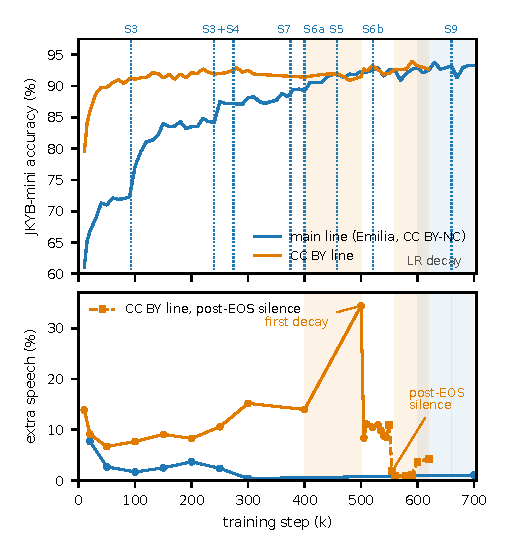
\includegraphics[width=\columnwidth]{fig_training_en.pdf}
\caption{Teachers during training (CFG 2.0). Top: reading accuracy rises when new synthetic data
arrives, not with more steps. Bottom: sentences with extra speech after the text. In the CC BY line,
data cleaning and decays did not remove it; supervising the frames after EOS did. Dotted: synthetic
sets entering the main line's mix (Table~\ref{tab:synth}; S3+: a larger share of S3). Shaded: decays.}
\label{fig:training}
\end{figure}

\textbf{Data, not steps.} The main teacher plateaued three times (70--72\%, 83.5--85\%, 87.5--88\%),
and each plateau ended only when a new synthetic set entered (Fig.~\ref{fig:training}). The
validation loss did not show the gains: it was the same at 93k and 100k steps while JKYB-mini rose by
5\pt. A final cosine decay (600k$\to$660k) added 0.6\pt{} on JKYB-mini and 4.6\pt{} on Aozora (JSUT
CER 2.86$\to$2.40\%). The CC BY teacher, with synthetic data from the start, reached 90\% at 35k
steps.

\subsection{How an utterance ends}\label{sec:end}
\textbf{Short chunks.} On 172 short texts the main teacher at 660k added speech after 58 and did not
stop on 22 (CER 28\%). A short stage with S9 at 1\% of the hours (40k steps, learning rate raised and
decayed again) fixed both within 5k steps (1 and 1, CER 4.8\%).

\textbf{Frames after EOS.} The CC BY teacher added fillers (``うん'', ``えー'') after 7--15\% of the
JKYB-mini sentences, 3--5$\times$ the main line; its first decay raised this to 34\%. Data fixes each
stopped near 7--11\%: trimming YODAS3 clip ends, re-checking YODAS3 by ASR, dropping fillers, even
removing YODAS3 (7.1\%, with speaker similarity 0.545$\to$0.500). Generating no frames after EOS gave
3.3\% instead of 8.8\%: most fillers were in the 5 frames the runtime adds. Upstream training masks
the loss after the last speech frame, so these frames are never seen. We append six frames of
digital silence (the Mimi latents of zeros) to every complete target and apply the flow loss to them;
the EOS target stays where speech ends. Within 10k steps extra speech fell from 10.9\% to 0.9\% (main
line 1.1\%), sentence CER from 3.6--3.9\% to 1.9\%, short-text CER from 11.8\% to 5.2\%, with no
change in EOS loss or speed. Late in the next decay fillers returned, now before EOS (4.3\% at 620k),
so the teacher is the 580k checkpoint.

\section{Distillation}\label{sec:distill}
\textbf{Guidance.} Without CFG the teacher read 1.2\pt{} worse, failed to stop more often and was
3.9\,LU quieter; scale 2.0 read best (93.0\% vs 90.5\% at 2.5). Since the runtime has no CFG, a copy
of the 24-layer teacher learns the frozen teacher's guided state $z_\varnothing+2(z_c-z_\varnothing)$
(MSE on the transformer output, heads frozen, 50k steps). It reads slightly better than the guided
teacher and is released as \texttt{japanese\_24l}.

\textbf{Depth.} The 6-layer student follows upstream's depth distillation: it starts from the
teacher's layers 0, 1, 2, 21, 22 and 23 (upstream found the outer layers the best seed) and learns
the guided state (main line: 42k + 120k steps; CC BY: 160k). On all of JKYB the students \emph{beat}
their teachers: 94.15 / 94.73\% against 92.97 / 93.68\% (main) and 93.93 / 93.96\% against 92.82 /
93.82\% (CC BY; prompts in rotation / jvs001, original decoder), as upstream's English student does
(WER 0.76 vs 0.82\%). They fail to stop more often (43 of 13,536 sentences against 6). In bfloat16 the
6-layer model runs 4.4$\times$ faster than real time on one CPU thread (24 layers: 1.4$\times$).

\textbf{Frames after EOS at release.} A level check of the clip ends (original decoder) showed that half of the 24-layer
CC BY model's short end sounds come after EOS (10.1\% of clips; 2.5\% cut while sounding). With 3
frames they drop to 7.9\% with 0.7\% cut (0 frames: 5.9\% but 16\% cut), so its config sets 3. The
6-layer model's sounds come before EOS (9.4--9.8\% at any setting) and listening found them
unobjectionable, so it keeps the default. With the CC BY decoder the released 24- and 6-layer models
end so in 6.4 and 8.9\% of the clips.

\section{Fine-tuning the decoder}\label{sec:decoder}
\textbf{Why.} Through Mimi, the kana CER of all JVS~\cite{jvs} read speech rises from 3.16\% to
5.45\%, mostly by consonants that change place (キ$\to$チ, ガ$\to$ダ). A consonant classifier gets
94.1\% from the latents but 92.0\% from the decoded audio: the decoder loses the information. We
train only the decode side (10.3M parameters), so the encoder, latents, language model and voice
prompts stay as they are, and the runtime loads the decoder from the same weight file.

\textbf{Main line.} Losses: multi-scale mel, MPD~\cite{hifigan} and MS-STFT~\cite{encodec}
discriminators, and a loss on the batch-averaged spectrum against tones at the stride frequencies
(multiples of 200\,Hz and 1.2\,kHz); data: 182\,h of synthetic speech and 60\,h of high-bitrate
Emilia. Every metric improved, yet listening rejected two decoders, for metallic consonants and a
pitch-locked high band: above 4\,kHz they made noise where recordings have harmonics. Holding that
band at the original decoder's output for the last 10k steps (\emph{keep4k}) fixed it by ear and
kept the gains (Table~\ref{tab:decoder}).

\textbf{The high band.} A research branch trained the band above 4\,kHz towards studio
recordings~\cite{hificaptain,jvnv}. Only UTMOSv2~\cite{utmosv2} (40\,Hz high-pass on every file)
agreed with all listening verdicts (UTMOS22~\cite{utmos}: rank correlation $-0.86$;
ViSQOL~\cite{visqol} ranked a rejected decoder first), and even it missed a mechanical sound. Harmonic
excitation from an F0 head sounded worse and needs new inference code; wider decoders changed
nothing. The predicted MOS of the training data set the order of the decoders, and averaging runs of
different recipes~\cite{soups} gave the best one, which uses NC and share-alike data.

\textbf{CC BY decoder.} It may use only the original Mimi, YODAS3 and the synthetic speech in CC BY
voices. YODAS3 clips are cut again at 24\,kHz from videos with audio up to 15\,kHz and high DNSMOS
(90k clips, 234\,h). Ranking clips by UTMOSv2 helped, by harmonic strength not. The base trains 70k steps from the original Mimi on 164\,h of YODAS3 and
116\,h of synthetic speech, discriminators included; four 10k-step runs then train the high band on
the top UTMOSv2 clips without band limits or clipping (7--14\,h) and are averaged. Two videos that listening revealed as synthetic
voices were left out. The result matches the best NC decoder in reconstruction and slightly exceeds
it in TTS (UTMOSv2 +0.35--0.42 over the original Mimi, speaker similarity 0.55$\to$0.65), and
listening could not tell the CC BY decoders from the best NC one.

\begin{table}[t]
\centering\footnotesize\setlength{\tabcolsep}{3pt}
\caption{Decoders on JVS reconstruction (10 speakers $\times$ 100 sentences). UTMOSv2 relative to
keep4k.}
\label{tab:decoder}
\begin{tabular}{@{}lrrrl@{}}
\toprule
Decoder & CER & Sim. & UTMOSv2 & Data\\
\midrule
Recording & 3.34 & -- & +0.400 &\\
Original Mimi & 5.44 & 0.698 & $-0.036$ &\\
keep4k (main release) & 4.70 & 0.779 & 0 & NC\\
Best average (research) & 4.74 & 0.784 & +0.397 & NC, SA\\
CC BY (\texttt{M2CH2\_soup4}) & 4.69 & 0.805 & +0.383 & CC BY\\
\bottomrule
\end{tabular}
\end{table}

\section{Released models}\label{sec:results}
Table~\ref{tab:results} compares the releases. Generated audio is transcribed with kana-whisper:
JKYB-Parakeet~\cite{jkyb,jkybp} (13,536 sentences, each with a tagged target; prompts from four JVS
speakers in rotation, or jvs001), its 1,500-sentence subset JKYB-mini, 1,000 Aozora ruby targets from
works not used for synthesis, 1,000 JSUT~\cite{jsut} sentences, zero-shot cloning of 10 JVS speakers
(kana CER and ECAPA similarity to the speaker's own recording of the sentence) and 172 short texts.
JVS and JSUT are never trained on. The stock package on CPU, loading the released files, matches
within noise (main line \texttt{japanese}: JKYB-mini 95.3\%, JSUT 2.15\%, JVS 1.70\% / 0.575).

\begin{table}[t]
\centering\scriptsize\setlength{\tabcolsep}{1.6pt}
\caption{Released models (GPU evaluation; L: layers; teachers with CFG 2.0). JKYB: all sentences,
prompts in rotation / jvs001. CER in \%. Short: did not stop / extra speech, of 172.}
\label{tab:results}
\begin{tabular}{@{}lrrrrrr@{}}
\toprule
Model & JKYB & mini & Aoz. & JSUT & JVS / sim. & Short\\
\midrule
\multicolumn{7}{@{}l}{\emph{Main line (CC BY-NC), decoder keep4k}}\\
6L & 94.75 / 94.84 & 95.1 & 71.3 & 2.28 & 2.32 / .577 & 0 / 1\\
24L & 94.32 / 94.49 & 94.5 & 71.2 & 2.28 & 2.13 / .586 & 0 / 1\\
\multicolumn{7}{@{}l}{\emph{CC BY line, CC BY decoder}}\\
6L & 94.77 / 94.49 & 94.9 & 70.7 & 2.14 & 2.18 / .651 & 0 / 2\\
24L & 94.36 / 94.85 & 94.9 & 70.3 & 2.13 & 2.47 / .645 & 0 / 0\\
\multicolumn{7}{@{}l}{\emph{Original Mimi decoder}}\\
Main 6L & 94.15 / 94.73 & 93.8 & 70.0 & 2.39 & 2.58 / .536 & 0 / 1\\
CC BY 6L & 93.93 / 93.96 & 94.3 & 69.0 & 2.40 & 2.47 / .560 & 0 / 1\\
CC BY 24L & 93.34 / 94.08 & 93.5 & 68.5 & 2.48 & 2.67 / .547 & 0 / 0\\
Main teacher & 92.97 / 93.68 & 93.3 & 69.4 & 2.66 & 3.05 / -- & 1 / 2\\
CC BY teacher & 92.82 / 93.82 & 92.7 & 67.9 & 2.58 & 2.45 / .546 & 0 / --\\
\bottomrule
\end{tabular}
\end{table}

With its own decoder the CC BY line, trained on half the data, reaches
the main line's accuracy. Both 6-layer models misread about 5\% of the JKYB
sentences, mostly rare readings and jukujikun.

\section{Discussion}
\textbf{What mattered.} First, \emph{coverage}: the model learns a reading only when it hears it
often enough, and synthetic speech from a TTS model that reads well, checked by ASR, is the cheapest
way to provide it, provided the check keeps the hard readings. Second, \emph{train what the runtime
does}: the frames after EOS, short chunks and the missing CFG each had to be supervised or distilled.
Third, \emph{metrics are not enough for the decoder}: every rejected decoder improved all of them.

\textbf{Limitations.} Scores are ASR-based with one seed, and JKYB-mini moves by about
$\pm$0.5--1\pt{} between evaluations. We ran no controlled ablation of the synthetic share, and the
synthetic speech carries Irodori's readings and style. The students fail to stop slightly more often
than the teachers, and 6--9\% of the CC BY clips end in a short, quiet sound.

\section{Conclusion}
A drop-in Japanese Pocket TTS needs no change to the runtime. Most of the gain came from the data:
web speech re-checked by ASR, matched loudness, and synthetic speech that covers rare readings.
Supervising the frames generated after EOS removed trailing fillers, distillation gave a 6-layer
model that reads better than its teacher, and a decoder fine-tuned on CC BY audio brought the CC BY
line level with the line trained with Emilia.

\section*{Acknowledgments}
We thank Kyutai for Pocket TTS and its training code, and the authors of Emilia, YODAS3, Irodori-TTS,
JKYB and its Parakeet edition, kana-whisper, JSUT, JVS, Hi-Fi-CAPTAIN, JVNV, UTMOSv2, Aozora Bunko,
Wikipedia, Tatoeba and the EDRDG dictionary files.

\begin{thebibliography}{99}\footnotesize
\setlength{\itemsep}{0pt}
\bibitem{pocket} M.~Orsini, S.~Rouard, G.~De~Marmiesse, V.~Volhejn, N.~Zeghidour, A.~Défossez.
Pocket TTS. \url{https://github.com/kyutai-labs/pocket-tts}, 2026.
\bibitem{calm} S.~Rouard, M.~Orsini, A.~Roebel, N.~Zeghidour, A.~Défossez. Continuous audio
language models. \emph{ICLR}, 2026.
\bibitem{mar} T.~Li, Y.~Tian, H.~Li, M.~Deng, K.~He. Autoregressive image generation without vector
quantization. \emph{NeurIPS}, 2024.
\bibitem{lsd} N.~M.~Boffi, M.~S.~Albergo, E.~Vanden-Eijnden. How to build a consistency model:
Learning flow maps via self-distillation. \emph{NeurIPS}, 2025.
\bibitem{cfg} J.~Ho, T.~Salimans. Classifier-free diffusion guidance. arXiv:2207.12598, 2022.
\bibitem{moshi} A.~Défossez et al. Moshi: a speech-text foundation model for real-time dialogue.
arXiv:2410.00037, 2024.
\bibitem{emilia} H.~He et al. Emilia: An extensive, multilingual, and diverse speech dataset for
large-scale speech generation. \emph{SLT}, 2024.
\bibitem{emilialarge} H.~He et al. Emilia: A large-scale, extensive, multilingual, and diverse
dataset for speech generation. arXiv:2501.15907, 2025.
\bibitem{ecapa} B.~Desplanques, J.~Thienpondt, K.~Demuynck. ECAPA-TDNN: Emphasized channel
attention, propagation and aggregation in TDNN based speaker verification. \emph{Interspeech}, 2020.
\bibitem{dnsmos} C.~K.~A.~Reddy, V.~Gopal, R.~Cutler. DNSMOS P.835: A non-intrusive perceptual
objective speech quality metric to evaluate noise suppressors. \emph{ICASSP}, 2022.
\bibitem{yodas} X.~Li et al. YODAS: YouTube-oriented dataset for audio and speech. \emph{ASRU}, 2023.
\bibitem{yodas3} W.~Chen, S.~Takamichi, S.~Shiota, S.~Fukayama, S.~Cornell, S.~Watanabe. YODAS v3:
Over 1 million hours of high-bandwidth, stereophonic, multilingual speech. \emph{Interspeech}, 2026.
\bibitem{silero} Silero Team. Silero VAD. \url{https://github.com/snakers4/silero-vad}.
\bibitem{whisper} A.~Radford et al. Robust speech recognition via large-scale weak supervision.
\emph{ICML}, 2023.
\bibitem{kanawhisper} SB Intuitions. \texttt{sbintuitions/kana-whisper}. Hugging Face.
\bibitem{yomi} Claude, T.~Mori. Teaching a flow-matching TTS to read kanji: Text-only
self-distillation of the text encoder of Irodori-TTS. Technical report, 2026.
\bibitem{jmdict} J.~Breen. JMdict: a Japanese-multilingual dictionary. \emph{COLING Workshop on
Multilingual Linguistic Resources}, 2004.
\bibitem{sentencepiece} T.~Kudo, J.~Richardson. SentencePiece: A simple and language independent
subword tokenizer and detokenizer for neural text processing. \emph{EMNLP (demo)}, 2018.
\bibitem{hifigan} J.~Kong, J.~Kim, J.~Bae. HiFi-GAN: Generative adversarial networks for efficient
and high fidelity speech synthesis. \emph{NeurIPS}, 2020.
\bibitem{encodec} A.~Défossez, J.~Copet, G.~Synnaeve, Y.~Adi. High fidelity neural audio
compression. \emph{TMLR}, 2023.
\bibitem{hificaptain} NICT. Hi-Fi-CAPTAIN corpus.
\url{https://ast-astrec.nict.go.jp/en/release/hi-fi-captain/}.
\bibitem{jvnv} D.~Xin et al. JVNV: A corpus of Japanese emotional speech with verbal content and
nonverbal expressions. \emph{IEEE Access}, 2024.
\bibitem{utmosv2} K.~Baba, W.~Nakata, Y.~Saito, H.~Saruwatari. The T05 system for the VoiceMOS
Challenge 2024. \emph{SLT}, 2024.
\bibitem{utmos} T.~Saeki et al. UTMOS: UTokyo-SaruLab system for VoiceMOS Challenge 2022.
\emph{Interspeech}, 2022.
\bibitem{visqol} M.~Chinen et al. ViSQOL v3: An open source production ready objective speech and
audio metric. \emph{QoMEX}, 2020.
\bibitem{soups} M.~Wortsman et al. Model soups: averaging weights of multiple fine-tuned models
improves accuracy without increasing inference time. \emph{ICML}, 2022.
\bibitem{jvs} S.~Takamichi et al. JVS corpus: free Japanese multi-speaker voice corpus.
arXiv:1908.06248, 2019.
\bibitem{jkyb} SB Intuitions. Joyo Kanji Yomi Benchmark.
\url{https://github.com/sbintuitions/Joyo-Kanji-Yomi-Benchmark}.
\bibitem{jkybp} Parakeet Inc. Joyo Kanji Yomi Benchmark, Parakeet Edition.
\url{https://github.com/Parakeet-Inc/Joyo-Kanji-Yomi-Benchmark-Parakeet-Edition}.
\bibitem{jsut} R.~Sonobe, S.~Takamichi, H.~Saruwatari. JSUT corpus: free large-scale Japanese
speech corpus for end-to-end speech synthesis. arXiv:1711.00354, 2017.
\end{thebibliography}
\end{document}
